
\section{System Demonstration}

During the conference, we plan to give an interactive demonstration of the 
{\system}'s capabilities.
We built a user interface to allow the user to interact with \system. 
We will allow the user to use tables from our NFL data set or political data
for campaign management queries.

Our demonstration will illustrate the following points: 
(1) The ability to perform statistical text analytics inside the DBMS.
(2) Query driven computation of analytics.
(3) The flexibility of our data sources by using structured data and text.
(4) Query execution over large amounts of text in real-time.
(5) Ability to perform textual analytics across multiple domains. \\

\begin{figure}
    \begin{center}
	   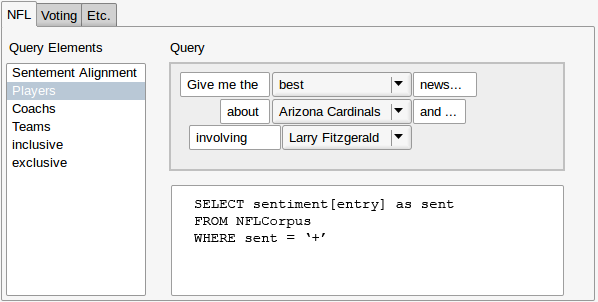
\includegraphics[scale=.35]{content/graphics/ui1.png}
	   \label{fig:ui1}
	   \caption{\system UI} 
	\end{center}
\end{figure} 

\noindent
\textbf{User Interface}\\
\system provides a web-based interface for interaction with the system.
The user interface displays the files and database statistics visible to
\system, as seen in an example mockup in Figure \ref{fig:ui1}. 
We allow customization of our example queries using a 
Mad Lib\footnote{http://en.wikipedia.org/wiki/Mad\_Libs} style interface.
The user can fill in the blank portions of the query data classes using the 
drop down list and filling in text boxes, or input their own custom queries.
The SQL for the query is presented to the user during graphical construction.
The execution time of a query is also visible to the user.\\

\begin{figure}
\begin{center}
	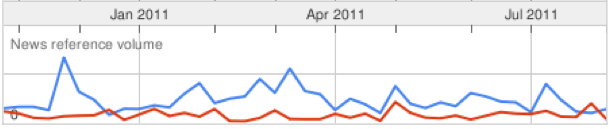
\includegraphics[scale=.35]{content/graphics/timeseries.png}
	\label{fig:timeseries}
	\caption{News over time H. Clinton vs J. Biden} 
\end{center}
\end{figure}


\noindent
\textbf{Other Domains}\\
Our running example has shown possible 
queries in the sports domain, but our system is also 
applicable in e-discovery, computational journalism, and 
campaign management.
Social networking sentiment has proven to be a leading indicator
for events such as the presidential elections \cite{o2010tweets}.
We will allow the user to perform query-driven 
exploration of real-time data using a query interface.
We will also provide pre-built 
queries to allow users see the running of real-time 
text analytic queries. As an example, a user may ask:

{\tt Who has more positive news in the twittersphere 
over the past 12 months `Hillary Clinton' or `Joe Biden'? }
\noindent
The result of this query
can be presented as a time series graph, shown in Figure \ref{fig:timeseries}.
Attendees are free to add new datasets from different domains to 
experiment with the abilities of \system.



